%        File: topology.tex
%     Created: Thu Nov 09 01:00 PM 2006 C
% Last Change: Thu Nov 09 01:00 PM 2006 C
%
% This file is part of Netsukuku
% (c) Copyright 2007 Andrea Lo Pumo aka AlpT <alpt@freaknet.org>
%
% This source code is free software; you can redistribute it and/or
% modify it under the terms of the GNU General Public License as published 
% by the Free Software Foundation; either version 2 of the License,
% or (at your option) any later version.
%
% This source code is distributed in the hope that it will be useful,
% but WITHOUT ANY WARRANTY; without even the implied warranty of
% MERCHANTABILITY or FITNESS FOR A PARTICULAR PURPOSE.
% Please refer to the GNU Public License for more details.
%
% You should have received a copy of the GNU Public License along with
% this source code; if not, write to:
% Free Software Foundation, Inc., 675 Mass Ave, Cambridge, MA 02139, USA.
%

\documentclass[a4paper]{article}
\usepackage{color,graphicx}
\usepackage{amsmath}
\usepackage{amsthm}
\usepackage{amssymb}
\usepackage{amsfonts}
\RequirePackage{ifpdf} % running on pdfTeX?
\ifpdf
\usepackage[pdftex]{hyperref}
\else
\newcommand{\href}[2]{ #1 }
\fi
\title{Netsukuku topology}
\author{http://netsukuku.freaknet.org\\AlpT (@freaknet.org)}
\begin{document}
\maketitle

\begin{abstract}
	In this document, we describe the fractal structure of the Netsukuku
	topology. Moreover, we show how it is possible to use the QSPN v2 on
	the high levels of the fractal.
\end{abstract}

\section{Preface}
\label{sec:preface}

We're assuming that you already know the basics of the QSPN. If not, read the
QSPN document first: \cite{qspndoc}.

\section{The general idea}
\label{sec:general_idea}

The aim of Netsukuku is to be a (physical) scalable mesh network, completely
distributed and decentralised, anonymous and autonomous.

The software, which must be executed by every node of the net, has to be
unobtrusive. It has to use very few CPU and memory resources, in this way it
will be possible to run it inside low-performance computers, like Access Points,
embedded devices and old computers.

If this requirements are met, Netsukuku can be easily used to build a worldwide
distributed, anonymous and not controlled network, separated from the
Internet, without the support of any servers, ISPs or control authorities.

\section{Basic definitions}

\begin{description}
	\item[Node] We call \emph{node} any computer that is hooked up to the
		Netsukuku network.
	\item[Rnode] stands for remote node: given a node X, it is any other
		node directly linked to X, i.e. it's a neighbour of X.
	\item[Map] A map is a file, kept by each node, which contains all the
		necessary information about the network, f.e. routes and nodes
		status.
\end{description}
Example:\\
\begin{figure}[h]
	\begin{center}
		\includegraphics[scale=0.5]{fig/segABC}
	\end{center}
	\caption{The nodes A,B and C}
\end{figure}
A is the rnode of B.\\
B is the rnode of A and C.\\
C is the rnode of B.

\section{Network topology}
\label{sec:net_topology}

A simple topology, which doesn't impose any structure on the network, can be
memorised with a simple map. In this map, all the information regarding the
nodes of the network have to be memorised. Surely, this kind of map cannot be
utilised by Netsukuku, because it would require too much memory.
For example, even if we store just one route to reach one node and even if
this route costs one byte, we would need 1Gb of memory for a network composed
by $10^9$ nodes (the current Internet).

For this reason, it's necessary to structure the network in a convenient
topology.

\subsection{Fractal topology}
\label{sec:fractal_topology}
\subsubsection{Level 1}
First of all we'll subdivide the network in groups of 256 nodes and we'll use
the following definitions:
\begin{description}
	\item[Gnode] means group node. It is a group of nodes, i.e. a set of
		nodes. Each node of the network belongs to just one gnode.\\
		A gnode contains a maximum of 256 nodes.\\
		By writing $n \in G$ we mean that the node $n$ belongs to the
		gnode $G$.
	\item[Bnode] stands for border node. It is a node which belongs to a
		gnode G, but that is also directly linked to at least one node
		of another gnode, i.e. some of its rnodes belongs to different
		gnodes than its.\\
		By writing $b \in G$ we mean that the bnode $b$ belongs to the
		gnode $G$.
\end{description}

Example:\\
\begin{figure}[h]
	\begin{center}
		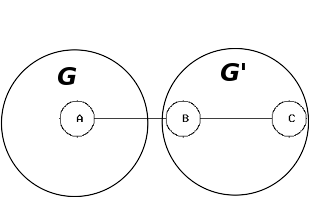
\includegraphics[scale=0.5]{fig/bnode}
	\end{center}
	\caption{The bnode A and B, belonging respectively to the gnode G and
	$G'$}
\end{figure}
$A \in G $, A is a node belonging to the gnode G, its rnode is B.\\
$B \in G'$, B is a node belonging to the gnode $G'$, its rnode is A.\\
A is a bnode of G, while B is a bnode of $G'$.

\subsubsection{Level n}
We further subdivide the network topology in \emph{groups of 256 groups of nodes}
and we continue to name them as gnode.\\
At this point, we repeat recursively this subdivision process until
we can group all the nodes of the network into a single gnode.

Doing so, we've structured the network in $n+1$ levels (from $0$ to $n$).\\
In the base level (level 0), there are 256 single nodes.\\
In the first level (level 1), there are 256 normal gnodes. Each of them
contains 256 single nodes.\\
In the second (level 2), 256 gnodes of level 1 forms a single \emph{group of
groups of nodes}.\\
In the third (level 3), there are 256 groups of 256 groups of 256 groups of
256 nodes.\\
Continuing in this way, we arrive at the last level (level $n$), where there
is a single group which contains the whole network.\\

The QSPN algorithm is able to operate independently on any level,
considering each gnode as a single node of level 0.
For this reason, we can view the Netsukuku topology as a fractal, where each
level is composed by single nodes.

\subsubsection*{Example}

Figure \ref{fig:fract_circle}\footnote{this figure has been taken from:
\href{http://www.ian.org/FX/Plugins.html}{http://www.ian.org/FX/Plugins.html}}
is an example of the fractal topology of Netsukuku.

\begin{figure}[h]
	\begin{center}
		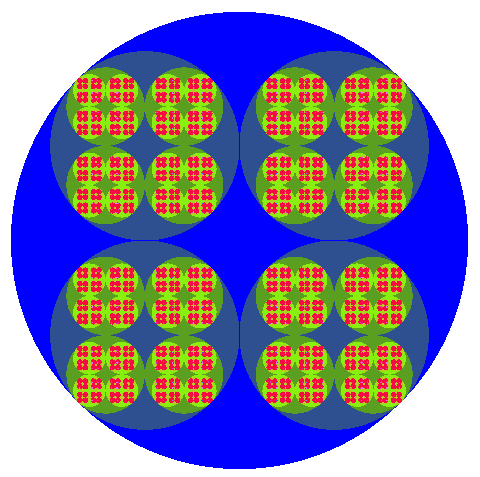
\includegraphics[scale=0.5]{fig/fractal_circle}
	\end{center}
	\caption{An example of the netsukuku topology structure}
	\label{fig:fract_circle}
\end{figure}

In this topology, each gnode contains four nodes, i.e. each group contains
four elements. The network is structured in 6 levels.\\
The red elements, are single nodes (level 0).\\
Four nodes forms a single group of nodes (level 1).\\
A single bright green circle is a 
				  group of groups of nodes (level 2).\\
The dark green circles are        groups of groups of groups of nodes (level 3).\\
The dark blue circle are          groups of groups of groups of groups of
nodes (level 4). \\
Finally, the bright blue circle is the gnode which contains the whole network
(level 5).

\subsubsection{Membership}
Let's assign a numeric ID to each (g)gnode, starting from the last level:
\begin{enumerate}
	\item in the last level ($n$) there's only one giant gnode, thus we assign
		to it the ID ``0''. Our global ID will be:
		\[
		0
		\]
	\item in $n-1$ there are 256 gnodes, which belongs to the gnode 0 of
		level $n$, thus we assign them the IDs from $0$ to $255$.
		The global ID becomes:
		\[
		0\cdot i\quad 0\le  i\le 255
		\]
	\item we repeat the step 2 recursively gaining an ID of this form:
		\[
		0\cdot i_{n-1}\cdot i_{n-2}\cdot \dots \cdot i_0 \quad 0\le i_j\le 255,\;0\le j\le n-1
		\]
	\item since the last level is always $0$, we'll omit it and we'll
		consider only the first $n$ levels.
\end{enumerate}
In a network with a maximum of $2^{32}$ nodes (the maximum allowed by the ipv4),
there would be five levels ($n=4$), where each gnode will be composed by 256 nodes.
Therefore, the ID will be in the usual IP form:
\[
0\dots255\cdot 0\dots255\cdot 0\dots255\cdot 0\dots255
\]
For example, a single node of level 0 of the network is:
\[
3\cdot 41\cdot 5\cdot 12
\]
That said, each gnode of the network belongs to only one combination of gnodes
of the various levels. In our previous example we have:
\begin{align*}
	&g_3=3\\
	&g_2=41\\
	&g_1=5\\
	&g_0=12
\end{align*}
where each $g_i$ corresponds to the gnode ID of the level $i$. Note that $g_0$
is the ID attributed to the single node, at level 0.

\subsection{Fractal map}
The advantages of using a fractal topology are clear.\\
The node $N$, instead of memorising information about each node of the whole
network, will keep only that regarding the gnodes where it belongs to.
Suppose the node $N$ had this ID:
\[
g_3\cdot g_2\cdot g_1\cdot g_0
\]
It will store in memory information regarding:
\begin{enumerate}
	\item the 256 single nodes which belongs to its same gnode of level 1,
		or in other words, the 256 nodes of the gnode $g_1$,
	\item the 256 gnodes gnodes which belongs to its same gnode of level
		2, of in other words, the 256 gnodes of the gnode $g_2$,
	\item finally, the 256 gnodes which belongs to the gnode $g_3$.
\end{enumerate}
Note that doing so, the node $N$ will be blind to all the other gnodes. For
example, it won't know any information regarding the single nodes which belong
to all the other gnodes of level 1 different from $g_1$.\\

Even with this lack of knowledge, as we'll see later, the node $N$ is still
able to reach all the other nodes of the network.
In conclusion, $N$ only needs $256n$ entries in its map, instead of $2^{32}$. 
To clarify the ideas suppose that each entry costs one byte. In the plain
topology we needed $4Gb$, while in the fractal one we just need $256\cdot 4\;
b= 1Kb$.

\subsubsection{IP v4 and v6}
Netsukuku is both compatible with ipv4 and ipv6.\\

In ipv4 there are a maximum of $2^{32}$ IPs, thus we have five levels $n=4$.\\
In ipv6 there are a maximum of $2^{128}$ IPs, thus $n=16$.

\subsubsection{Internal and external map}
For simplicity we divide the map of the node $N$, in the \emph{internal map} and in
the \emph{external} one.  The internal map contains information regarding the
nodes belonging to $g_1$. The external map describes all the other levels of
the topology.

\subsubsection{Bnode map}
The bnode map of the node $N$  contains the information regarding the bnodes
of each level where $N$ belongs.
Some examples to clarify the ideas:\\

suppose that $N = g_3\cdot g_2\cdot g_1 \cdot g_0$
\begin{itemize}
	\item a bnode of level 0 is a single node linked with two nodes of two
		different gnodes of level 1.
	\item the bnodes of level 0, known by $N$, are only that which belong
		to the gnode $g_0$. Thus are all the nodes of $g_0$ which are
		linked to at least a gnode different from $g_1$.
\end{itemize}

\subsection{CIDR routing}
The QSPN, for each level, will build the routes necessary to connect each
(g)node to all the other (g)nodes of the same level. The routes will be saved
in the maps of each node.\\

If the node $N=g_3\cdot g_2\cdot g_1 \cdot g_0$ wants to reach a node $M$ which
belongs to different gnodes, f.e. $M=g_3\cdot g_2\cdot h_1 \cdot h_0$, it will
add a CIDR\cite{CIDR} route in the routing table of the kernel:\\
\emph{all the packets whose destination is $g_3\cdot g_2\cdot h_1 \cdot 0\dots
255$ will be forwarded to the gateway $X$}.\\

We'll see later how the gateway $X$ is chosen.

\section{Tracer Packets in high levels}
In the QSPN document \cite{qspndoc}, we've seen how a Tracer Packet works in a
network composed by single nodes, i.e. a gnode of level 0. \\
We'll now study its way of working on higher levels.

\subsection{A gnode is a node}
In the abstract sense a single node is an entity which:
\begin{enumerate}
	\item receives input from its links
	\item stores it in its memory
	\item computes it
	\item and sends the output of the computation over some of its links
\end{enumerate}
Thus any other entity which performs the same operations can be thought as a
single node.\\
A gnode $G$ can act as a single node too.
\begin{enumerate}
	\item A bnode $I$, which belongs to $G$, receives an input from its
		links. We call $I$ the ingress (b)node.
	\item this input is flooded to all the nodes, of any level, of the
		gnode. The nodes will memorize the information contained in
		the input.\\
		Note that the flood is not a TP. The flooded pkt will be
		received only once by each node.
	\item A bnode $O$, of the same gnode, which is different from $I$,
		receives the flooded input and computes it.
		We call $O$ the egress (b)node.
	\item The bnode $O$ sends the output of its computation to its
		external links, i.e. avoiding those links which connect it to
		nodes of $G$ or to the same gnode which sent the input to $I$.
\end{enumerate}

\subsubsection{Example of a wandering TP}
Consider the network in figure \ref{fig:qspn_g3}.\\
\begin{figure}[h]
	\begin{center}
		\includegraphics[scale=0.5]{fig/qspn_g3}
	\end{center}
	\caption{The gnodes $G_1$, $G_2$ and $G_3$}
	\label{fig:qspn_g3}
\end{figure}
$G_1$, $G_2$, $G_3$ are gnodes of level 1. $A_1$ and $A_2$ belong to $G_1$. $B_1$ and $B_2$ belong to
$G_2$. $C_1$ belongs to $G_3$.\\

Suppose the node $A_1$ sends a Tracer Packet in level 1 
\footnote{Note that any node can send a TP in any level. In this case, we are
considering $A_1$, which is a bnode, to simplify the example}. 
The following will happen:
\begin{enumerate}
	\item The TP is flooded in $G_1$.
	\item $A_2$ receives the TP and appends in it the ID of the gnode
		$G_1$.
	\item $A_2$ sends the TP to $B_1$.
	\item $B_1$ receives it, updates its maps and floods it in $G_2$.
	\item All the node belonging to $G_2$ will receive the TP, updating their
		maps.
	\item This same procedure is reiterated from step 2, i.e. $B_2$ receives
		the TP, appends the ID of $G_2$ and so on until $C_1$ receives
		it.
	\item $C_1$, noticing that its gnode hasn't any links to other gnodes
		than $G_2$, will bounce back the TP to $B_2$ and at the same
		time will flood $G_3$.
	\item The TP, with the same procedure, will return back to $A_1$,
		completing the TP cycle.
\end{enumerate}

\section{QSPN v2 in high levels}
In order to use the $Q^2$ (QSPN v2) in high levels, we need to be sure that a TP,
flooded inside a lower gnode, will reach once and only once all the nodes of
the same gnode. Moreover, a good metric needs to be defined for the high
levels: what is the rtt (Round-Trip Time) and bandwidth capacity of the link
between the two gnodes $G_1$ and $G_2$?

\subsection{Endless loops}
Consider the situation in figure \ref{fig:3bnodes}.
\begin{figure}[h]
	\begin{center}
		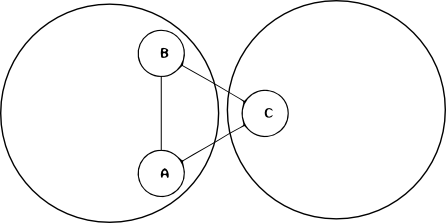
\includegraphics[scale=0.6]{fig/3bnodes}
	\end{center}
	\caption{Three bnodes, forming a cycle}
	\label{fig:3bnodes}
\end{figure}
A and B are bnodes of the node $G_1$, while $C$ is a bnode of the gnode $G_2$.
Suppose C sends a TP to B. B floods it inside $G_1$, thus $A$ receives it. At
this point, $A$ sends the packet to all its external links, and thus to $C$.
$C$ will send the packet again to $B$ and the cycle will continue.\\

This situation can be avoided if an ingress bnode, before forwarding a packet to a an
external gnode $F$, checks if the packet has already traversed $F$ itself. If
it has, the bnode won't forward it to $F$.

\subsection{Route Efficiency Measure}
We will refer to REM (Route Efficiency Measure), as a value characterising the
quality of a route. REM can be calculated in various ways, f.e. by taking in
account the total rtt and the bw capacity of the route. We suppose that
the REM value of a normal route/link has been already defined. 

\subsubsection{Gnode metric}
The REM value of a route, whose hops are gnodes and single nodes is defined as
follow.
\begin{enumerate}
	\item The REM value of the route $x\rightarrow y$ is $E(x\rightarrow
		y)$. The following condition must be respected:
		\begin{enumerate}
			\item 
		The REM of a route has to be associative:
		\[
		REM(x\rightarrow y\rightarrow z)=REM(x\rightarrow
		y)+REM(y\rightarrow z)
		\]
		\item The REM of the loopback route must be ``zero'':
			\[
			REM(z\rightarrow z)+REM(x\rightarrow y)=REM(x+y)
			\]
		\end{enumerate}
	\item Let $G$ be a gnode, $x$ one of its nodes and $x \rightarrow G$ the
		link between the node and the gnode. $x \rightarrow G$ can be
		thought as the set of all the routes, which connect $x$ to
		each node of $G$. The REM value of $x \rightarrow G$, should
		tell the ability of the node $x$ to reach a generic node of
		$G$. For this reason, we define $E(x \rightarrow G)$ as the
		arithmetic mean of the REM value of all the routes, connecting
		$x$ to every node of $G$. In symbols:
		\begin{align*}
		&n=|G|,\quad g_i\in G\\
		&E(x\rightarrow G)=\frac{\sum_{i=1}^n E(x \rightarrow g_i)}{n}
		\end{align*}
		where $g_i$ is a node of $G$, and $n$ is the number of nodes
		of $G$.
	\item Let $A=\{a_1, \dots,a_j\}$ and $B=\{b_1,\dots,b_k\}$ be two sets 
		of nodes, then:
		\begin{align*}
		E(A \rightarrow  B)&=
		\frac{\sum_{i=1}^j\sum_{e=1}^k E(a_i \rightarrow b_e)}{jk}\\
		&=
		\frac{\sum_{i=1}^j {\sum_{e=1}^k E(a_i \rightarrow b_e) \over
		k}}{j}\\
		&=
		\frac{\sum_{i=1}^j E(a_i \rightarrow B)}{j}
		\end{align*}
		$E(A \rightarrow B)$ indicates the cost of moving from a
		generic node of $A$ to a generic node of $B$.
	\item \label{p4}
		\begin{enumerate}
			\item Let $G=\{g_1,\dots,g_n\}$ be a gnode. We consider it as a set of
				nodes.
			\item Let $H$ be a gnode bordering with $G$.
			\item Let $x \in H$, i.e. let $x$ be a node of $H$.
			\item Let $B_G=\{g_1',\dots,g_j'\}$ be the set
				of the bnodes of $G$ and $B_H=\{h_1', h_2',
				\dots,h_j'\}$ the set of bnodes of $H$ such
				that $g_i'$ is connected with with $h_i'$ for
				$i=1,\dots,j$.
		\end{enumerate}
		We define the REM value $E(x\rightarrow G)$
		as the arithmetic mean of the REM value of all the routes, connecting
		$x$ to every node of $G$, such that only one bnode of type $h_i'$ and
		one of type $g_i'$ is contained in each route.\\
		The REM value of the link $x\rightarrow G$ can be calculated as
		follow:\\
		\begin{eqnarray*}
		E(x \rightarrow \{g_1',\dots,g_j'\})&=&
				\frac{\sum_{i=1}^j E(x \rightarrow h_i' \rightarrow g_i')}
						{j}\\
				&=&
				\frac{\sum_{i=1}^j E(x \rightarrow
				h_i')+E(h_i' \rightarrow g_i')}{j}\\
		E(\{g_1',\dots,g_j'\}\rightarrow G)&=&
				\frac{\sum_{i=1}^j E(g_i'\rightarrow G)}{j}\\
		(*)\;\;\;E(x\rightarrow G)&=&
			E(x \rightarrow \{g_1',\dots,g_j'\}) + E(\{g_1',\dots,g_j'\}\rightarrow G)
		\end{eqnarray*}
		The equation $(*)$ corresponds to the searched arithmetic mean. 
		It is convenient to calculate it in this form, because we can
		split its computation in two independent phases: the
		computation of $E(x\rightarrow B_G)$ and that of
		$E(B_G\rightarrow G)$. Doing so, the node $x$, to compute
		$E(x\rightarrow G)$,  will only need
		to calculate $E(x\rightarrow B_G)$. The $E(B_G\rightarrow G)$
		value, which it can't calculate since it is an external node
		to G, will be calculated and sent by the same $B_G$ bnodes.
		Here follow the proof of equation $(*)$.
		\begin{proof}
			\label{proofrem1}
			For simplicity, by writing $\overline{xy}$ we will indicate the route $x
			\rightarrow y$.\\
			All the routes from $x$ to $G$ are:
			\begin{align*}
				&\overline{x h_1  g_1'  g_1},\;\; \overline{x
				h_1  g_1'g_2},\;\;\dots,\;\; \overline{x h_1
				g_1'  g_n}\\
				&\overline{x h_2  g_2'  g_1},\;\; \overline{x
				h_2  g_2'g_2},\;\;\dots,\;\; \overline{x h_2
				g_2'  g_n}\\
				&\qquad \vdots\\
				&\overline{x h_j  g_j'  g_1},\;\; \overline{x
				h_j  g_j'g_2},\;\;\dots,\;\; \overline{x h_j
				g_j'  g_n}
			\end{align*}
			As we can see, there are $n$ routes which passes from
			a single bnode $h_i'$ and $g_i'$. Since there are $j$
			bnodes, the total number of routes is $jn$.

			The arithmetic mean of their REM is:
			\[
			\frac{\sum_{k=1}^n \sum_{i=1}^j
			E(\overline{xh_i'g_i'g_k})}{jn}
			\]
			By the associative property of REM we can write:
			\[
			\frac{\sum_{k=1}^n \sum_{i=1}^j
			E(\overline{xh_i'g_i'})+E(\overline{g_i'g_k})}{jn}
			\]
			that is the same of:
			\begin{align*}
			\frac{n\sum_{i=1}^j E(\overline{xh_i'g_i'})+\sum_{k=1}^n \sum_{i=1}^j
			E(\overline{g_i'g_k})}{jn}=\\
			\frac{n\sum_{i=1}^j E(\overline{xh_i'g_i'})}{jn}+\frac{\sum_{k=1}^n \sum_{i=1}^j
                        E(\overline{g_i'g_k})}{jn}=\\
			\frac{\sum_{i=1}^j E(\overline{xh_i'g_i'})}{j}+\frac{\sum_{k=1}^n \sum_{i=1}^j
                        E(\overline{g_i'g_k})}{jn}
			\end{align*}
			The last identity is exactly what we were looking for:
			\begin{align*}
			E(x \rightarrow
			\{g_1',\dots,g_j'\})&=\frac{\sum_{i=1}^j
			E(\overline{xh_i'g_i'})}{j}\\
			E(\{g_1',\dots,g_j'\}\rightarrow
			G)&=\frac{\sum_{k=1}^n
			\sum_{i=1}^jE(\overline{g_i'g_k})}{jn}\\
			E(x\rightarrow G)&=
			E(x \rightarrow \{g_1',\dots,g_j'\}) +
			E(\{g_1',\dots,g_j'\}\rightarrow G)\\
			&= \frac{\sum_{i=1}^j
			E(\overline{xh_i'g_i'})}{j}+\frac{\sum_{k=1}^n
			\sum_{i=1}^jE(\overline{g_i'g_k})}{jn}
			\end{align*}
		\end{proof}
	\item Under the same assumption of point \ref{p4}, we add only the
		following: let $X=\{x_1,\dots,x_r\} \subseteq H$.
		We define $E(X\rightarrow G)$ as the average of the REM value
		of all routes connecting $x_i \rightarrow G$ for
		$i=1,\dots,r$. The constraint imposed on the routes
		$x_i \rightarrow G$ have been already defined in point
		\ref{p4}. This definition is equivalent to:
		\[
		E(X\rightarrow G) = \frac{\sum_{i=1}^rE(x_i\rightarrow G)}{r}
		\]
		\begin{proof}
			In the precedent proof (\ref{proofrem1}) we've seen
			that the average of the REM value of the routes $x\rightarrow G$ is
			\[
			\frac{\sum_{k=1}^n \sum_{i=1}^j
			E(\overline{xh_i'g_i'g_k})}{jn}
			\]
			thus in this case, it's just a matter of adding
			another summation:
			\begin{align*}
				& \frac{\sum_{e=1}^r \sum_{k=1}^n
				\sum_{i=1}^jE(\overline{x_eh_i'g_i'g_k})}{jnr}=\\
				&\frac{\sum_{e=1}^r\left(
				\frac{\sum_{k=1}^n \sum_{i=1}^j
				E(\overline{x_eh_i'g_i'g_k})}{jn}
				\right)}{r}=\\
				&\frac{\sum_{e=1}^rE(x_e\rightarrow G)}{r}
			\end{align*}
		\end{proof}
		%%%% TODO CONTINUE HERE:
		%% \dots\rightarrow X\rightarrow Y\rightarrow \dots
\end{enumerate}


\subsubsection{REM in a Tracer Packet}
Each link contained in a TP contains its relative REM value. Consider the TP
$D \leftarrow  C \leftarrow   B \leftarrow   A$, where each hop is a gnode.
The REM value saved in the packet are computed and appended hop by hop:
\begin{description}
	\item[1. $a'\leftarrow A\;$] The egress bnode $a'$ of $A$, having received the
		TP, computes\\ $E(A)=E(\{a_1',\dots,a_j'\}\rightarrow A')$ as
		described above. $\{a_1',\dots,a_j'\}$ are all the egress bnodes of
		$A$ bordering on $B$. The computed value $E(A)$ is saved in the
		packet. The TP is then forwarded to $B$.
	\item[2. $b_i\leftarrow b'\leftarrow a' \leftarrow A\;$] The generic node
		$b_i \in B$ receives the TP. Utilising the saved $E(A)$ value,
		it computes $E(b_i\rightarrow A)$ as explained before, but doesn't modify the
		packet. $b_i$ will use the $E(b_i\rightarrow A)$ value to
		update and order its routes.\\
		The packet continues to be forwarded.
	\item[3. $b'' \leftarrow b_i \leftarrow b' \leftarrow a' \leftarrow
		A\;\;$] The egress bnode $b'' \in B$ receives the TP. $b''$, as
		the other nodes of $B$, computes and saves for itself the
		$E(b''\rightarrow A)$ value. Moreover, $b$ does the following:
		\begin{itemize}
			\item it computes $E(\{b_1',\dots,b_j'\}\rightarrow B')$
				and appends it in the packet as the value
				$E(B)$,
			\item it computes \[
				E(\{b_1'',\dots,b_k''\}\rightarrow
				\{b_1',\dots,b_j'\} \rightarrow A)+E(A)
				\]
				and saves this value in the packet overwriting
				$E(A)$
		\end{itemize}
		The packet continues to be forwarded.
	\item[4. $c_i\leftarrow b''\leftarrow \dots\;$] The generic node $c_i \in
		C$ receives the packet. It computes \\$E(c_i \rightarrow B)$
		using the saved $E(B)$ value, without modifying the packet.
	\item[5. $c''\leftarrow c_i \leftarrow b''\leftarrow \dots\;$] The egress
		bnode $c'' \in C$ receives the packet and computes for itself
		$E(c''\rightarrow B)$. It computes also $E(C)$ saving it in
		the packet.\\
		Finally, it finally overwrites $E(B)$ with
		$E(\{c_1'',\dots,c_k''\}\rightarrow B)$.
		The packet continues to be forwarded.
	\item[6. $\dots\leftarrow \dots\;$] This same procedure is re-iterated
		from step 4 until the TP arrives at the last gnode $D$.
\end{description}

\subsubsection*{Example of REM in a TP}
See figure \ref{fig:gmetric}.
\begin{figure}[h]
	\begin{center}
		\includegraphics[scale=0.4]{fig/gmetric}
	\end{center}
	\caption{Gnodes metric example}
	\label{fig:gmetric}
\end{figure}

These will be the respective REM values saved in a TP which has traversed the
whole net:
\begin{align*}
	E(\mathbf{G}_3)&=\frac{E(\overline{C_1 \mathbf{G}_3})+E(\overline{C_2 \mathbf{G}_3})
	+E(\overline{C_3 \mathbf{G}_3})}{3} \\ 
	E(\overline{\mathbf{G}_2\mathbf{G}_3})&=
	\frac{
		E(\overline{A_2 \mathbf{\mathbf{G}}_2  B_1 C_1})+
		E(\overline{A_2 \mathbf{\mathbf{G}}_2  B_2 C_2})+
		E(\overline{A_2 \mathbf{\mathbf{G}}_2  B_3 C_3})
	     }{3} + 
	     E(\mathbf{\mathbf{G}}_3)\\
	E(\mathbf{G}_1\mathbf{G}_2\mathbf{G}_3)&= 
		E(\overline{\mathbf{\mathbf{G}}_1 A_1 A_2})+
		E(\mathbf{G}_2\mathbf{G}_3)
\end{align*}

\subsection{Unique flood}
Suppose that a TP has been flooded inside the gnode $G$.
Suppose also that the node $n \in G$ receives two duplicate packets.\\
The $Q^2$ instructs the node $n$ to keep forwarding only the interesting packets.
A packet, which is a perfect copy of a packet already received, is always
uninteresting. Therefore, the node $n$ will drop the second copy of the
received TP. 

However, in this case the node $n$ should not consider the REM
values saved in the TP, because two TPs, which have crossed the same
gnodes in the same order, might have different REM values.
\\

In conclusion, whenever two or more TPs, which have crossed the same high level
route, are received by a node of $G$, only one of them will be forwarded. In
this way, the successive nodes will receive only one copy of the same packet.

\section{Network dynamics}
When a part of the network changes considerably, the maps of the involved
levels must be updated.

\subsection{Radar}
Every node has its own radar, which periodically sends a broadcast request to
all its (physical) near nodes. By collecting the replies, the radar is able to
determine the active rnodes of the node and the quality of its links.

\subsection{Level 0}
In level 0, a QSPN is sent every time a node joins the network, dies or every
time the change of the quality of a link exceeds a predefined delta value.
The QSPN is sent by the nodes noticing the changes, i.e. by the rnodes of the
mutated node. In this case the QSPN is restricted to level 0, and thus it cannot
escape from the gnode where it has been originated.

In order to prevent false positives, the rnodes of the mutated node won't
immediately send the QSPN, but will wait a small amount of time. If the change
persists, they will send the QSPN.

\subsection{Level n}
In high levels the bnodes are responsible to start the new QSPN.
The bnode $b \in G$ will send a QSPN in the level of $G$, every time the value
$E(G)$ or\\$E(B_G\rightarrow B_R)$ changes substantially.

The bnode can notice the change of $E(G)$ by inspecting the QSPN of lower
levels, which are sent inside $G$.
When the quality of the routes to reach the internal nodes of G varies, the $E(G)$
value will change too. If the variation exceeds a predefined delta, the bnode
will send a QSPN in the level of $G$, to inform the other gnodes that the links
passing through $G$ have now a different efficiency.

The bnode, instead of sending immediately the QSPN, will wait for a small
time, using a timer. During this wait, if it receives any other information about a
new variation of $E(G)$, it will resets the timer, waiting for a second time,
and it will increment the variation counter.\\
If the variation counter reaches the threshold value or if no more information
regarding $E(G)$ are received, then the bnode will send the QSPN.

This strategy is adopted to avoid false positives and to normalize the case
when $E(G)$ varies frequently. Thus if $E(G)$ varies four times in a minute,
only one QSPN will be sent, not four.

The same applies for the variation of $E(B_G\rightarrow B_R)$, where $B_G$ are
the bnodes of $G$ linked to the bnodes $B_R$ of the gnode $R$, which is any
bordering gnode of $G$. Only significant variations of $E(G\rightarrow R)$ are
considered. For examples, if $G$ and $R$ are connected by $20$ bnodes, when
only one of the bnode dies, the $E(G\rightarrow R)$ will (generally) vary lightly.

\subsection{Hooking phase}
A new node joins the network when it has been able to create at least one
physical link to an active Netsukuku node and when it has correctly executed
the hooking procedure. In this paragraph, we describe loosely the hooking
phase of a new node.

Suppose that the node $n$ has established a physical link to at least one Netsukuku
node. In order to become an active Netsukuku node, $n$ has to \emph{hook} to
its rnodes.

During the hook, $n$ will exchange vital information with its rnodes,
it will choose its new IP and it will finally become part of a gnode.

The hook procedure is formed by these general steps:
\begin{enumerate}
	\item The node $n$ chooses an IP in the range of $10.0.0.1 \le IP \le
		10.0.0.255$.
	\item It launches the first radar to see what its rnodes are. If not a
		single node is found, it creates a new gnode and ends hooking
		phase.
	\item At this point, $n$ asks to its nearer rnode the list of all the
		available free nodes presents inside the gnode of the rnode.\\
		If the rnode rejects the request (the gnode might be full),
		the node $n$ contacts another rnode.
	\item $n$ chooses an IP from the received list of free nodes and sets
		it on its network interface.
	\item $n$ will then download the external map from the same rnode.
		Looking at the external map, it will be able to determine if
		it has to create a new gnode. If it has, it creates it and
		ends the hooking.
	\item $n$ gets the internal and the bnode map from the same rnode.
	\item $n$ launches a second radar and updates its routing table.
\end{enumerate}


\subsection{Gnode hook}
When a node creates a new gnode, it will choose a random gnode ID, and thus
a random ip.\\
Suppose that two isolated gnodes get the same gnode ID. When they will be
linked, they'll enter in conflict.\\
The solution to this problem is to let each new gnode hook as a normal node
would. You can find more information about this in the NTK\_RFC 001\cite{gnodecontiguity}.

%%%%%%%%%%%%%%%%%%%%  TODO %%%%%%%%%%%%%%%%%%%%%

%bnode map
%ext map  (sizeof)
%int map  (sizeof)
%

%%%%%%%%%%%%%%%%
% Bibliography %
%%%%%%%%%%%%%%%%

\begin{thebibliography}{99}
	\bibitem{qspndoc} QSPN document:
		\href{http://netsukuku.freaknet.org/doc/main\_doc/qspn.pdf}{qspn.pdf}
	\bibitem{ntksite} Netsukuku website:
		\href{http://netsukuku.freaknet.org/}{http://netsukuku.freaknet.org/}
	\bibitem{CIDR} CIDR routing:
		\href{http://en.wikipedia.org/wiki/Classless\_Inter-Domain\_Routing}{Classless\_Inter-Domain\_Routing in Wikipedia}
	\bibitem{gnodecontiguity} NTK\_RFC 001:
		\href{http://lab.dyne.org/Ntk\_gnodes\_contiguity}{Gnode contiguity}
\end{thebibliography}
\newpage

\begin{center}
\verb|^_^|
\end{center}
\end{document}
